\documentclass[11pt,a4]{article}
\usepackage[cm]{fullpage}
\usepackage{graphicx}
\usepackage{subfigure}
\usepackage{epsfig}
\usepackage{epstopdf}
\begin{document}

\begin{figure}[h]
\centering
    \includegraphics[width=0.49\textwidth]{MAX}
    \includegraphics[width=0.49\textwidth]{REST}
    \includegraphics[width=0.49\textwidth]{TBP}
    \includegraphics[width=0.49\textwidth]{JUND}
\caption{Distribution of the distances from all true MPBSs to the center of the closest region predicted by segmentation-based methods for the cell line HeLa-S3. All HMM Models were trained with data from H1-hESC and K562 cell lines.}
\label{fig:boxplot.HeLaS3.fdr_4.1}
\end{figure}

\begin{figure}[h]
\centering
    \includegraphics[width=0.49\textwidth]{STAT1}
    \includegraphics[width=0.49\textwidth]{GABP}
    \includegraphics[width=0.49\textwidth]{FOS}
    \includegraphics[width=0.49\textwidth]{USF2}
\caption{Distribution of the distances from all true MPBSs to the center of the closest region predicted by segmentation-based methods for the cell line HeLa-S3. All HMM Models were trained with data from H1-hESC and K562 cell lines.}
\label{fig:boxplot.HeLaS3.fdr_4.2}
\end{figure}

\begin{figure}[h]
\centering
    \includegraphics[width=0.49\textwidth]{JUN}
    \includegraphics[width=0.49\textwidth]{E2F4}
    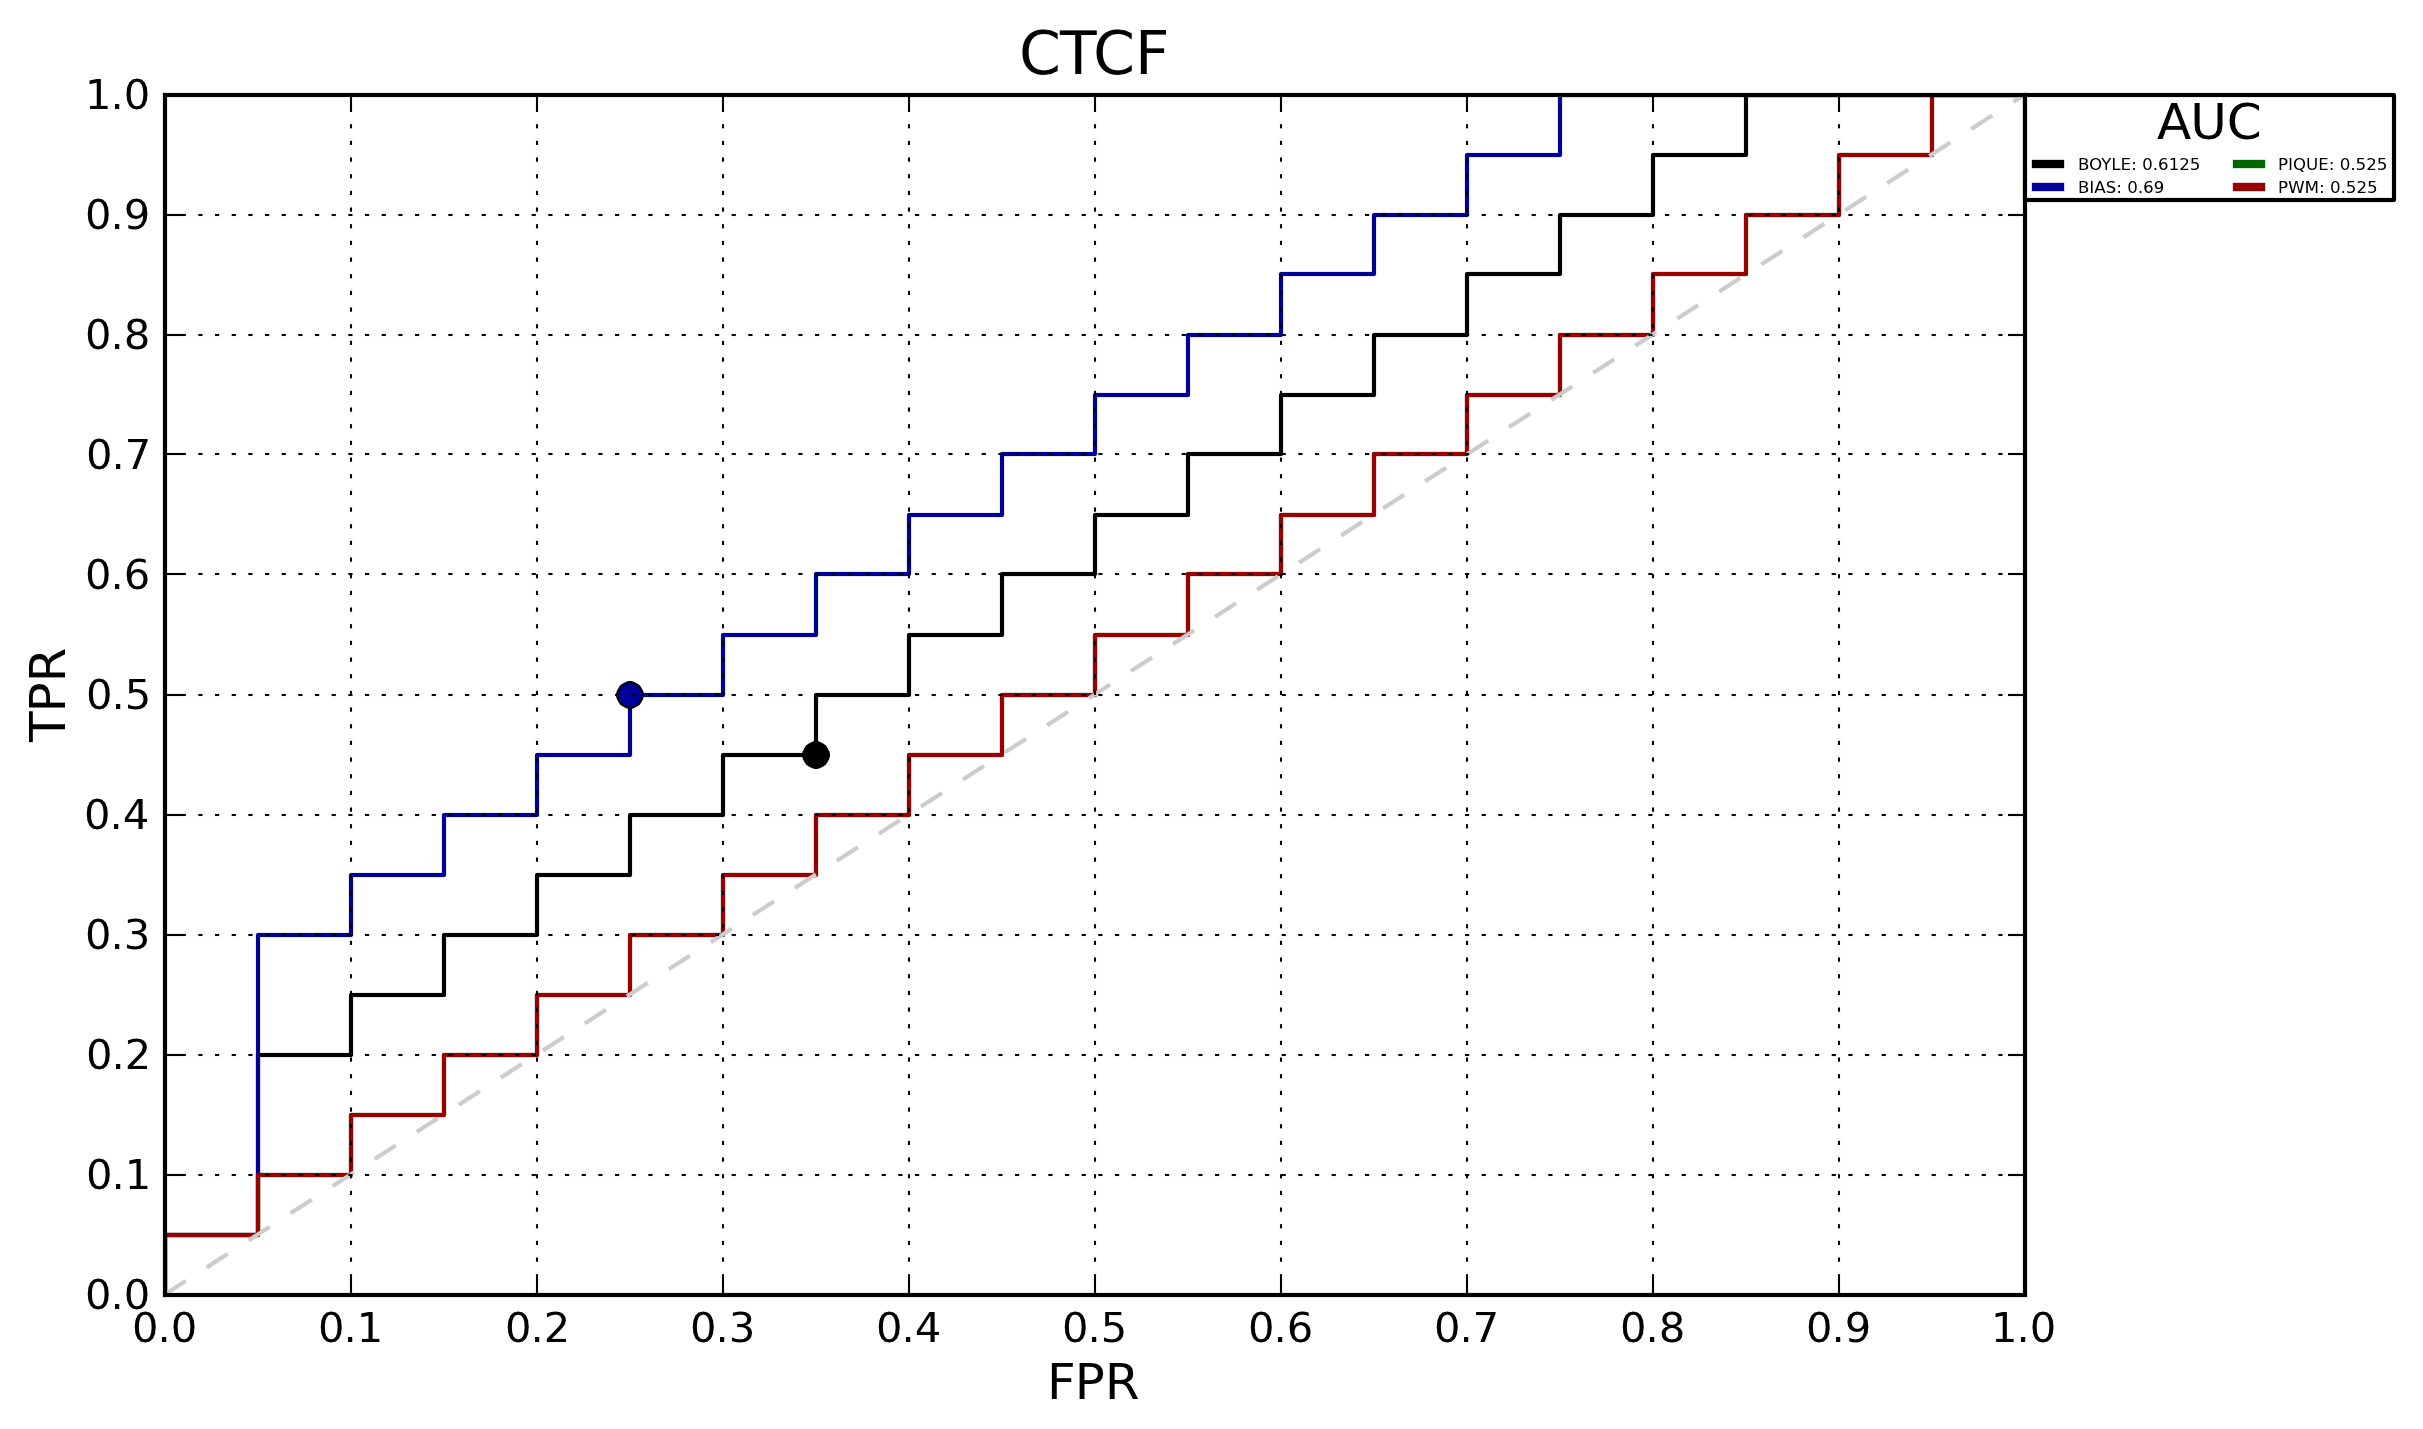
\includegraphics[width=0.49\textwidth]{CTCF}
    \includegraphics[width=0.49\textwidth]{MAFK}
\caption{Distribution of the distances from all true MPBSs to the center of the closest region predicted by segmentation-based methods for the cell line HeLa-S3. All HMM Models were trained with data from H1-hESC and K562 cell lines.}
\label{fig:boxplot.HeLaS3.fdr_4.3}
\end{figure}

\begin{figure}[h]
\centering
    \includegraphics[width=0.49\textwidth]{ELK1}
    \includegraphics[width=0.49\textwidth]{MYC}
    \includegraphics[width=0.49\textwidth]{NFYB}
    \includegraphics[width=0.49\textwidth]{NRF1}
\caption{Distribution of the distances from all true MPBSs to the center of the closest region predicted by segmentation-based methods for the cell line HeLa-S3. All HMM Models were trained with data from H1-hESC and K562 cell lines.}
\label{fig:boxplot.HeLaS3.fdr_4.4}
\end{figure}

\begin{figure}[h]
\centering
    \includegraphics[width=0.49\textwidth]{fdr_4}
    \includegraphics[width=0.49\textwidth]{RAD21}
    \includegraphics[width=0.49\textwidth]{ZNF143}
    \includegraphics[width=0.49\textwidth]{P300}
\caption{Distribution of the distances from all true MPBSs to the center of the closest region predicted by segmentation-based methods for the cell line HeLa-S3. All HMM Models were trained with data from H1-hESC and K562 cell lines.}
\label{fig:boxplot.HeLaS3.fdr_4.5}
\end{figure}

\begin{figure}[h]
\centering
    \includegraphics[width=0.49\textwidth]{CEBPB}
    \includegraphics[width=0.49\textwidth]{NFYA}
    \includegraphics[width=0.49\textwidth]{BRCA1}
    \includegraphics[width=0.49\textwidth]{E2F6}
\caption{Distribution of the distances from all true MPBSs to the center of the closest region predicted by segmentation-based methods for the cell line HeLa-S3. All HMM Models were trained with data from H1-hESC and K562 cell lines.}
\label{fig:boxplot.HeLaS3.fdr_4.6}
\end{figure}

\end{document}